\documentclass{article}

% Now also available outside of Overleaf at the following
% https://github.com/usna-roboroach-2021/ew401-fa2020-roboroach

% Any word on if they prefer IEEE journal format or old ES401?
% Don't worry about formatting - when the content is in I can
% do formatting by setting up a style file. 

\usepackage{graphicx}
\usepackage[utf8]{inputenc}

% Can we insert a "pre-title" that says EW401 Final Report?

\title{The RoboRoach}
\author{Midshipman 1/C Alexis Pak and Midshipman 1/C Brooklyn Pritchard\thanks{Authors are with the Department of Weapons, Robotics, and Control Engineering at the United States Naval Academy}}
% HOW DO I INCLUDE CONTACT INFO?

\begin{document}
\maketitle

\begin{figure}[ht!]
\centering

\includegraphics[scale=0.5]{logo.png}

\label{fig:logo}
\end{figure}

% INCLUDE AFTER THE FIGURE: 
    %A Capstone Project Report Submitted to the Faculty of The Weapons, Robotics and Control Engineering Department
    %United States Naval Academy, Annapolis, Maryland

    %Course:  EW401
    %Faculty Advisor: Asst Prof Dennis Evangelista
    %Department Chair: Prof Brad Bishop

    %date comes last
    \date{September 2020}

\tableofcontents

\begin{abstract}
\par Though our initial goal is to control the movements of a cockroach by creating a neural interface to stimulate it’s antennae, we also have a much broader goal for our project in the WRC department. Our problem statement is: To create a simple and repeatable lab that teaches students the process of scientific inquiry. It must fall under the maximum budget for a lab and teach some state of the art technique for studying organisms. Our four metrics for evaluating our project’s overall performance are simple, short, relevant, and convenient. The design that scored the highest in these metrics was the Build Your Own RoboRoach project. It earned a 2 in simple because though there are some givens with the lab, creating a RoboRoach requires some background knowledge in the major in topics like PWMS, duty cycles, computer vision and more. It earned a 1 in short because we estimated that it would take 5 lab sessions for a Midshipman to complete. It earned a 4 in relevant because it teaches students how to test and create a hypothesis. Lastly, it earned a 3 in convenience because we predicted that a professor could set up this lab within 1 hour.  Our RoboRoach will wear a PCB similar to the Backyard Brains backpack. Our backpack will consist of a TinyPico and a set of electrodes. The TinyPico contains all the individual components needed to execute the same tasks as the Backyard Brains backpack. The user will designate a direction via a game controller which will send the command via bluetooth signal to the backpack, which then sends a current to a specific electrode (left or right) and that electrical stimulation causes the roach to turn left or right. We plan on using Windows as our computing platform with Python and Arduino IDE as our programming languages. After meeting with TSD, we created a comprehensive parts list and determined which items to order and which were already available in-house. After crafting our budget, we estimated a total of \$14,040 for labor, \$14,040 for overhead, and \$614.24 for parts. 
\end{abstract}

% If it is easier, we can split these into different files to make
% it quicker to find the right bit to edit too. 
\section{Introduction}
\subsection{Customer Background}
\par The Roboroach Capstone customer is Professor Levi Devries, a professor in the WRC department. Professor Devries was a double major in Physics and Math and also got his Masters in Aerospace Engineering from UMD. Though his experiences with Biomechanical projects are few and far between, Professor Devries is very interested in developing a new lab in the WRC curriculum because he wants to reinforce ideas being taught in early level courses while providing a new and helpful lab. From our first interview, we delved deeper into this idea, discussing how we could offer a lab in the early curriculum as well as a follow on to the 1/C EW485E Biomechanics elective. We also developed our initial thoughts for our functionality, metrics, and objectives. During our second interview, we finalized our top four metrics which were: simple, short duration, relevancy, and statistical significance. 

\subsection{Additional Background Research}

\par The RoboRoach project could be extremely beneficial in the biomechanics realm as well as in everyday life. If we can program insects and control their motions or even have computer vision through the insects, we could use them in the military to carry out reconnaissance missions that would be too dangerous for humans. The learning outcomes could also be used in many different concentrations, including practicing controlling robots and having them execute certain tasks. Our additional background research is primarily focused on related projects that shared similar inspiration with our idea. 

\bigskip

\par The article "Minimuscles Let Amputees Control A Robot Hand With Their Minds" is centered around a robotic prosthetic hand. 
In short, the robot prosthetic hand taps into nerve signals in the arm to allow locomotive control and transmits brain commands through a wire. It creates mini muscles in the arm by bundling lots of small fibers to make new finger muscles. This article served as motivation for our project because we are looking to explore and model cockroach neurophysiology. Understanding cockroach neuromechanics could help us learn about human neuromechanics, in ways that are too invasive to try with humans or vertebrate animals. ***INCLUDE CITATION***

\bigskip

\par In "Bio-Inspired Non-Cooperative Multi-Robot Herding", a team created dog-like robots to herd non-cooperative sheep. The problem with using regular dogs for herding is that dogs are often unable to coordinate their motions to herd the sheep as a group. The purpose of the project was to create a safer alternative to other kinds of herding with finer control. The team created a controller that had the desired position for each robo-dog and used a proportional feedback controller to find the ideal velocity of the dogs based on its mapping. This project served as motivation for our project because we are also looking to achieve direction control over our subjects. Although the organisms and means by which we will be conducting our experiments are very different, the use of a proportional feedback controller could be applicable to our project in achieving autonomous control. ***INCLUDE CITATION***

\bigskip

\par Our last source of additional motivation is an article titled "Rapid Inversion: Running Animals And Robots Swing Like A Pendulum Under Ledges". In this project, a team observed how geckos and cockroaches use their hind legs as grappling hooks when swinging over ledges. Its ultimate goal was to create a robot to aid in Search and Rescue missions by using similar techniques to maneuver through rubble or tough terrain, or help with aid post natural disasters. It designed a robot called Dynamic Autonomous Sprawled Hexapod (DASH) to simulate this maneuver that both geckos and cockroaches perform. This project served as motivation for our project because this team's goal is also an application of our project. Because cockroaches are so agile and sturdy, with a human interface, they could also be used to aid in Search and Rescue missions or help with aid post natural disasters.***INCLUDE CITATION***

\section{Problem Statement}

\subsection{Problem Statement}
\par We aim to create a simple and repeatable lab that teaches students the process of scientific inquiry. It must fall under the maximum budget for a lab and teach some state of the art technique for studying organisms.

\begin{figure}[ht!]
\centering
\includegraphics[scale=0.25]{lab.JPEG}
\caption{WRC Students working on a lab in ES200}
\label{fig:hollywood}
\end{figure}

\subsection{Functions}
\par Our design should teach students how to create and test hypotheses and introduce a new lab that is exciting and non-traditional to the WRCE core labs. More specifically, students completing the lab should

\begin{itemize}
  \item Form a testable hypothesis
  \item Formulate a way to test their hypothesis
  \item Write a program that sends current to the electrodes
  \item Simulate the PCB's effect on a cockroach
  \item Perform surgery on a cockroach
  \item Achieve directional control over the cockroach
  \item Observe the cockroach's behavior
  \item Evaluate their original hypothesis based on the results
\end{itemize}

\subsection{Constraints}
\par We had 2 major constraints: The lab must teach some state of the art technique for studying organisms and the total cost of the lab must fall under the maximum budget for a lab. The lab must teach some state of the art technique for studying organisms because the biological aspect is what makes this lab different from all of the existing WRCE core labs. If the lab does not meet this constraint, it fails to fulfill its original purpose. The total cost of the lab must fall under the maximum budget for a lab because it needs to be repeatable. This lab will not be a feasible option to include in the WRCE curriculum if it is not as or less affordable than existing labs.

\subsection{Objectives, Pairwise Comparison Chart, and Weightings}
\par We break our objectives down into two main categories for this project- time conscious and repeatable. Under time conscious, we have the objectives simple and short. For simple, we are making sure that it is feasible for this lab to be completed by Midshipmen. For the objective of short, we want this lab to be executable in 4 lab sessions or less. Moving to the repeatable branch, we have the objectives relevant and convenient. The relevancy objective is to measure the ability that the lab gives the student to create and test a hypothesis while getting useful data from it. Convenience is measured by how easy it is for the lab to be set up by the professor. We allowed our customer to weight these objectives, and from this we created a pairwise comparison chart which is shown in \ref{fig:pcc}. 

\begin{figure}[ht!]
\centering
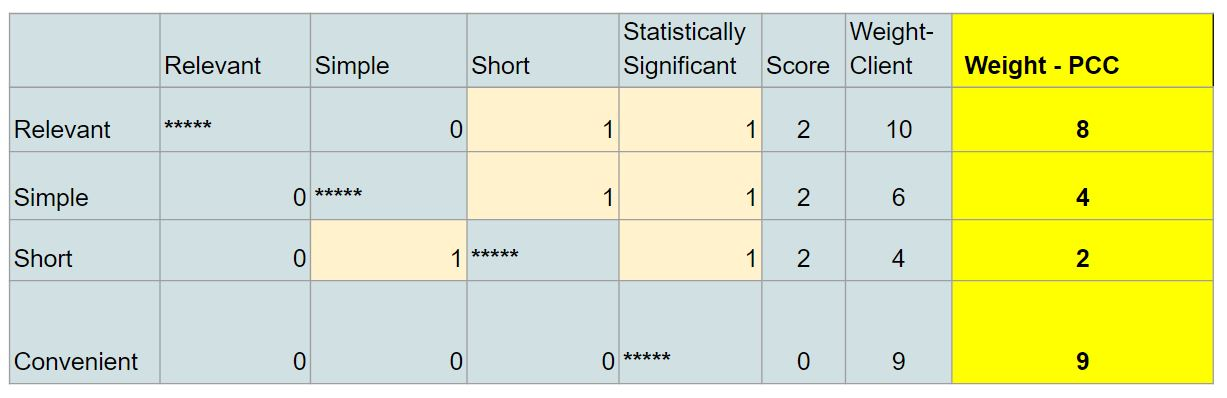
\includegraphics[scale=0.55]{PCC.JPG}
\caption{Pairwise Comparison Chart}
\label{fig:pcc}
\end{figure}

\subsection{Metrics}
\par The four highest weighted objectives for our project were simple, short, relevant, and convenient. We weighted each of them from 0-4 based on how they satisfied our customers desired outcomes. For simple, we looked at the level of understanding and training it took to complete the lab and weighted it accordingly. A 0 would be extremely difficult, requiring a graduate level education, while a 4 would require a technical background equivalent to that of a freshman undergraduate student. For the short metric, we gave a range of acceptable time that the lab could be completed in. It would score a 0 if it lasted for up to 600 minutes, or 6 lab periods, and a 4 if it lasted for less than 400 minutes or four lab periods. For the relevancy of the lab, we looked at how the students would be able to learn from this lab as well as achieve decisive results from it. The project would receive a 0 if it did not allow the students to test or create a hypothesis as well as not allowing them to achieve decisive results in their reports. A 4 would be given if they can successfully create and test a hypothesis as well as have decisive results that allow them to reflect on the project in their reports. Lastly, we looked at the convenience of the lab. We ranked it with a 0 if the lab caused the professor to spend weeks in advance prepping for the lab, and a 4 if the lab setup can by achieved by the professor in thirty minutes or less. We believe that with all of these metrics taken into account, we can properly address our problem statement by creating a simple and repeatable lab that teaches students the process of scientific inquiry by studying an organism.

\begin{figure}[ht!]
\centering
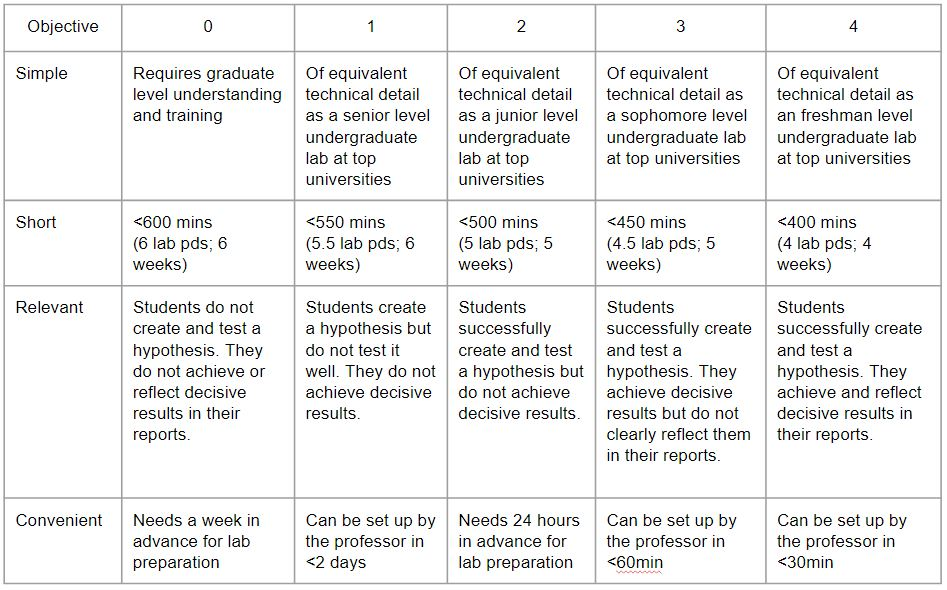
\includegraphics[scale=0.4]{metrics.JPG}
\caption{Metrics}
\label{fig:metrics}
\end{figure}

\section{Related Work}

% Also I'll help you guys do citations etc so don't worry about fixing those yet
\par The first related project we researched referred to controlling cows with virtual fencing. In ``Virtual Fences for Controlling Cows'', a team developed a moving virtual fence algorithm to herd cows \cite{butler2004virtual}. The intended market for this product is animal farmers or anyone who might need to herd animals. Because herding is a very labor intensive activity, the product aimed to eliminate the need for physical fences on farms. Their virtual fence methodology can be used to monitor grazing behavior in order to create models that lead to better land and pasture utilization, effectively optimizing the resource utilization, providing automation support, and easing the activities of animal farmers. The team made a smart collar for each cow in the herd, equipped with GPS, PDA (computer), wireless networking, and a sound amplifier. The animal is given the boundary of a virtual fence as a polygon specified by its coordinates and the GPS tracks its location against the polygon. As the animal approaches the boundary, a sound stimulus whose volume is proportionate to the distance from the boundary goes off. The team created static boundaries for grazing by leaving the polygon boundary as is, and dynamic boundaries for herding by slowly moving the polygon boundary in the desired direction. One lesson learned for our project is that the current moving speed of the test subject may influence the effect of the stimulus. Another lesson learned is that there are numerous ways to stimulate movement, such as emulating a behavior of a natural predator. We may incorporate the same approach with data collection as the team did, in that we would time how long it took the test subject to respond to the stimulus in the way we desire, but also take into account how often they respond in the way we desire. We did not see any specific shortcomings that they should have avoided or that we should avoid in the future. 

\bigskip

\par The second research article we looked was relating to controlling Hawkmoths. In ``Wireless Stimulation of Antennal Muscles in Freely Flying Hawkmoths Leads to Flight Path Changes'', the team used radio controlled, programmable, miniature stimulators to alter the pitch angle, flight speed, and flight altitude of hawkmoths \cite{hinterwirth2012wireless}. Though the intended user or market is not specified in the article, we believe that this product would appeal to researchers looking for a deeper understanding of neurophysiology within insects and subsequently humans. The goal of this product was to alter the flying behavior of a hawkmoth by stimulating its antennal mechanosensors. The team used \emph{Manduca sexta}, hawkmoths, as their test subject. Electrical stimuli were delivered to extrinsic antennal muscles via tiny electrodes injected to a dorsomedial location near each antennal rim. A miniature stimulator board delivered 2.8-3V square-pulse signals of 50 percent duty cycle and varying frequencies. A transmitter, communicating with the stimulator board wirelessly, was connected to a computer running software that stipulated the antennal muscles every 5 seconds. A high-speed video camera filmed the moth, and the team used a custom MATLAB digitizing software to extract the tip and base coordinates of the stimulated antenna and calculate deflection angles for each frame. One lesson learned for our project is that, at least for hawkmoths, stimulation of extrinsic muscles leads to antennal deflections while at rest. This article implies that this is true for all creatures with antennae, so we can expect similar results with a cockroach. Another lesson learned is that variation in electrode placement leads to slightly different recruitment of mechanosensors, so we will be extremely precise and deliberate in our measurements before we insert electrodes. The electrical stimulation aspect of this experiment will be very similar to that of ours. We will attempt to stimulate the same parts of the antennae for a cockroach that this team did for a hawkmoth. We also plan to use high-speed video cameras to observe our roaches so we will likely take a similar approach in the way we calculate the change in movement upon stimulation. Based on this article, it seems the best way to induce change in motion is by electrically stimulating the antennae. Furthermore, the best way to get consistent results is by ensuring identical electrode placement in all the test subjects. 

\bigskip

\par Lastly, we researched a more broad experiment on Automated insect robots. In ``Kinect-based System for Automated Control of Terrestrial Insect Biobots'', the team demonstrated neural stimulation techniques to control the motion of Madagascar hissing cockroaches \cite{whitmire2013kinect}. Though there is no intended user or market directly stated, we believe that researchers who want to learn more about achieving a neural interface with organisms or even teachers who want to incorporate biology into traditional technology-only labs could benefit from this study. It is widely recognized that biological systems have a highly optimized nature that is extremely difficult to replicate in synthetic robots. The goal of this study was to take an alternative approach. Rather than creating a synthetic robot, the team harnessed roaches and electrically stimulated their antennae to create biological robots (biobots). The team used a Kinect camera and test bed to contain and monitor the roach. The team created software to perform image processing on the live feed from the Kinect. The software was given a predefined path, a set of waypoints for the roach to follow. The strategist would compare the direction of the roach’s movement to the nearest waypoint at regular intervals. If the vectors differed by more than 25 degrees, the roach was given a stimulation pulse to correct the deviation. Each trial, the roach was placed right in front of the start path in the test bed, facing the direction of the first waypoint. The computer vision system detected the roach and automatically began directing it along the path. A National Instruments Data Acquisition Device interfaces with a digital potentiometer in conjunction with a microcontroller and transmitter to send a pulse-modulated signal to the receiver on the roach’s ``backpack''. The roach’s backpack consists of a receiver and microcontroller, which interface with the electrodes implanted in its antennae. One lesson learned from this study is that longer stimulation times generally led to a more pronounced turn by the insect. Another lesson learned is that, while a shorter duration of stimulation improved the ability of the system to make the roach follow the line, too short a duration could cause the next stimulus to preempt the desired reaction from the original stimulus. This experiment is very close to what we aim to achieve in our project. We will probably take the same approach in conducting our trials, making the roach follow a set of way points and stimulating it on a regular basis if it strays too far from the desired path. We will also take into account their stimulus durations and PWM duty cycles. The authors wrote that they did not optimize the surgical procedure or stimulation parameters such as number of waypoints or pulse durations. We will be careful not to repeat these shortcomings.

\bigskip

\begin{figure}[ht!]
\centering
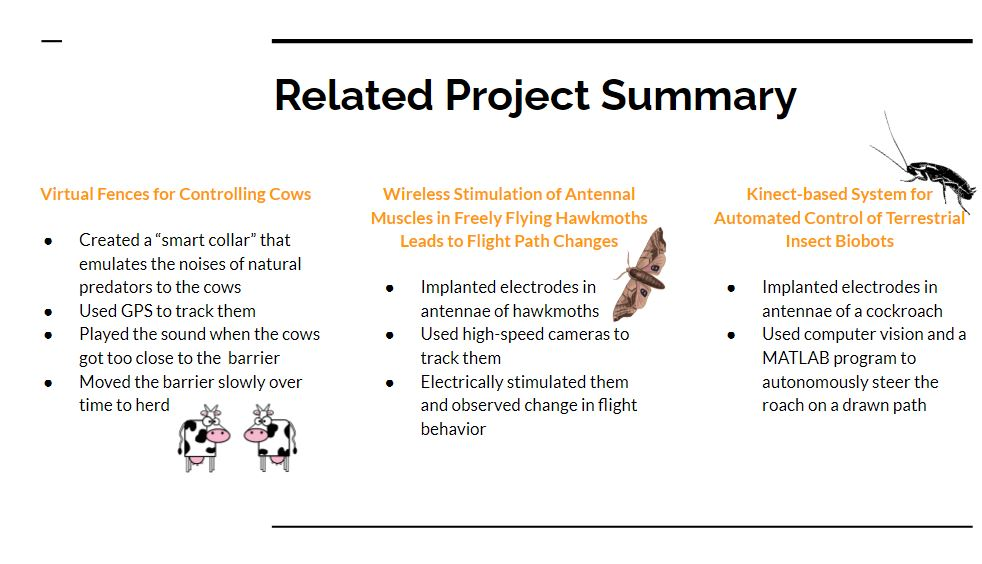
\includegraphics[scale=0.45]{relatedwork.JPG}
\caption{Summary of Related Work}
\label{fig:relatedwork}
\end{figure}

\section{Conceptual Designs}

\subsection{Concept 1: Wireless Stimulation of Hawkmoths}
\par For this project, students would implant electrodes in antennae of hawkmoths, electrically stimulate them, and use high-speed cameras to track and observe changes in flight behavior. By our metrics defined in the earlier section, we awarded this project 1 point in simple, 1 point in short, 4 points in relevant, and 3 points in convenient. It earned only 1 point in simple because, in order to successfully achieve directional control over a moth, students would need to have thorough understanding of the microcontroller, digitizing software, PWM, duty cycles, and computer vision. Moreover, flight control over a moth is far more difficult to control than simple left or right turns. Flight accounts for movement in the X, Y, and Z directions, and also pitch and yaw. We felt that this lab was of equivalent technical detail as a senior level undergraduate lab at top universities. It earned only 1 point in short because we estimated that, between surgery, programming, stimulation, and observations, students would need about 5 lab sessions (or 500 minutes) to complete the lab. It earned 4 points in relevant because it can effectively teach students how to create and test a hypothesis. The lab is very open-ended once the student achieves a successful interface with the moth, so it is not solution dependent. The students can test nearly any hypothesis approved by their professor. Finally, it earned 3 points in convenience because we estimated that, between bringing in surgery and observation materials and building the electrode sets and PCBs beforehand, the Professor should be able to set this lab up in less than an hour.

\begin{figure}[ht!]
\centering
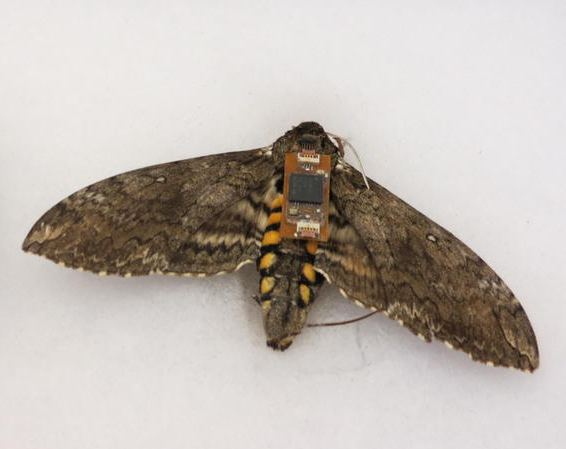
\includegraphics[scale=0.45]{moth.png}
\caption{Wireless Stimulation of Hawkmoths Conceptual Drawing}
\label{fig:concept1}
\end{figure}

\begin{figure}[ht!]
\centering
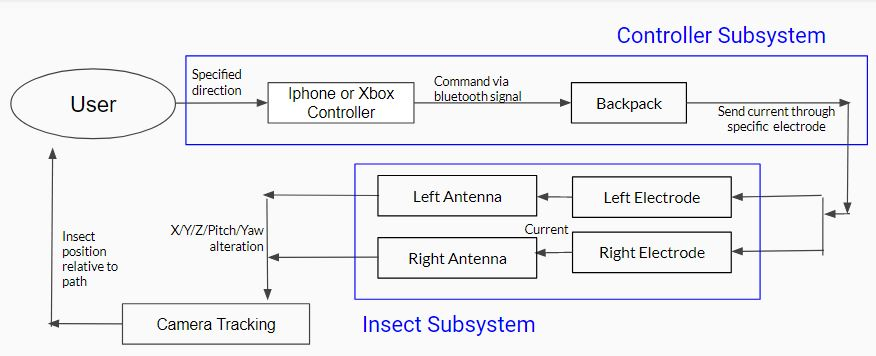
\includegraphics[scale=0.45]{fbd1.JPG}
\caption{Wireless Stimulation of Hawkmoths FBD}
\label{fig:FBD1}
\end{figure}

\subsection{Concept 2: Backyard Brains RoboRoach Kit}
\par For this project, professors would order multiple RoboRoach kits from Backyard Brains. Students would follow the Backyard Brains detailed instructions and use the corresponding phone application to achieve control over left and right turns on a cockroach. By our metrics defined in the earlier section, we awarded this project 4 points in simple, 4 points in short, 1 points in relevant, and 4 points in convenient. This lab earned a 4 in simple because the kit provides extremely detailed instructions on the surgery and how to use the app. Almost everything is done for the student. Therefore, we believe this lab to be of equivalent technical detail as an freshman level undergraduate lab at top universities. We awarded it a 4 in short because, given the simplicity, we estimated that less than 4 lab sessions (400 minutes) would be needed to complete this lab. It earned only 1 point in relevant because, while it does introduce some principles of neuromechanics, there is no coding or inquiry for the students. They are given everything they need to achieve directional control. The only step they are taking that is not in the directions is observation. We believe that students may create a hypothesis for this lab, but will not be able to test it very well since they only followed pre-made instructions and did not create the original code that sends current to the cockroach's antennae. Finally, this lab earned a 4 in convenience because the teacher really only needs to bring in the roaches and the kits as preparation for this lab, which can easily be done in less than 30 minutes.

\begin{figure}[ht!]
\centering
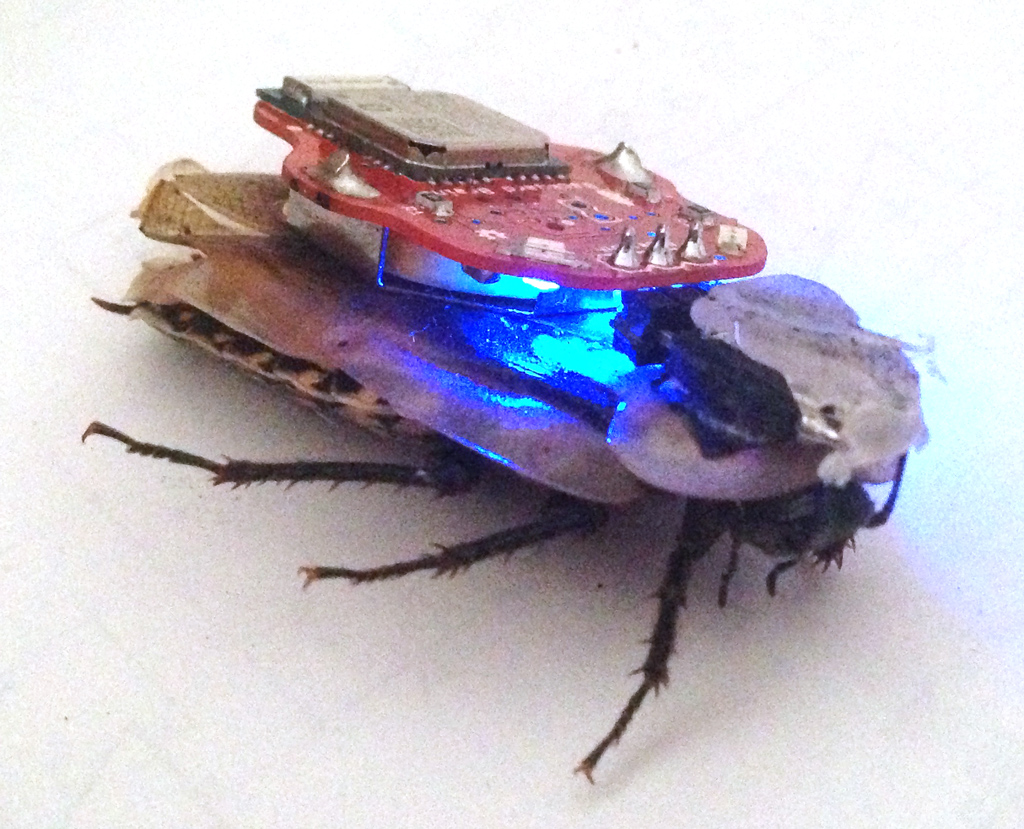
\includegraphics[scale=0.15]{roboroach.png}
\caption{Backyard Brains RoboRoach Kit Conceptual Drawing}
\label{fig:concept2}
\end{figure}

\begin{figure}[ht!]
\centering
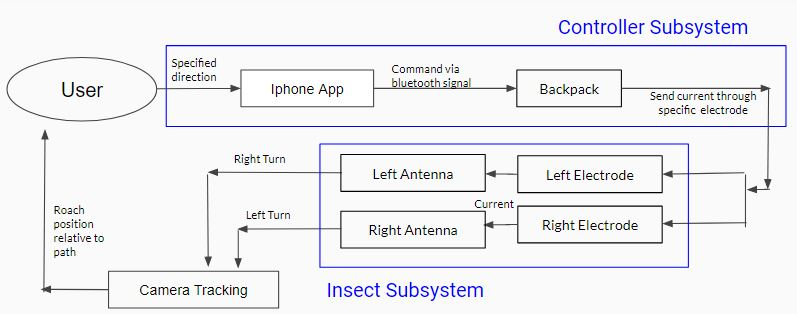
\includegraphics[scale=0.45]{fbd2.JPG}
\caption{Backyard Brains RoboRoach Kit FBD}
\label{fig:FBD2}
\end{figure}

\subsection{Concept 3: Make Your Own RoboRoach}
\par For this lab, professors would create the electrode sets and PCBs for the students, but the students would be responsible for the coding, control, and surgery of their cockroaches. Similar to the Backyard Brains Roboroach kit, the students would use electrical stimulation to make the cockroach turn left or right. However, it differs in that it offers students more room for error and learning since they are responsible for coding the PCB and sending the current to the antennae. By our metrics defined in the earlier section, we awarded this project 2 points for simple, 1 point for short, 4 points for relevant, and 3 points for convenient. It earned 2 points for simple because there are some givens, but the students still need a decent amount of background knowledge in the major to feel comfortable doing this lab. They should be familiar with PWM, duty cycles, and computer vision, which makes this lab of equivalent technical detail as a junior level undergraduate lab at top universities. It only earned 1 point for short because, given the ample freedom and opportunity to explore, fail, and learn using scientific inquiry, we estimated that students would need 5 lab periods (500 minutes) to complete this lab. We awarded 4 points for relevant because it effectively teaches students how to create and test a hypothesis without being solution dependent. Because students have full control over how they code their PCBs, they can manipulate their PCBs and their cockroaches to perform anything they hypothesize. It earned a 3 in convenient for the same reason as the hawkmoth lab- we estimated that, between bringing in surgery and observation materials and building the electrode sets and PCBs beforehand, the Professor should be able to set this lab up in less than an hour.

\begin{figure}[ht!]
\centering
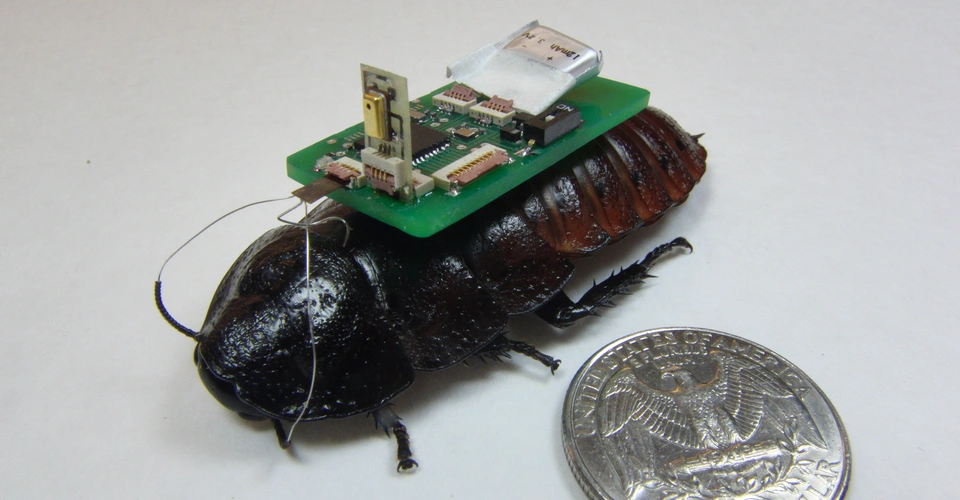
\includegraphics[scale=0.25]{myo.png}
\caption{Make Your Own RoboRoach Conceptual Drawing}
\label{fig:concept3}
\end{figure}

\begin{figure}[ht!]
\centering
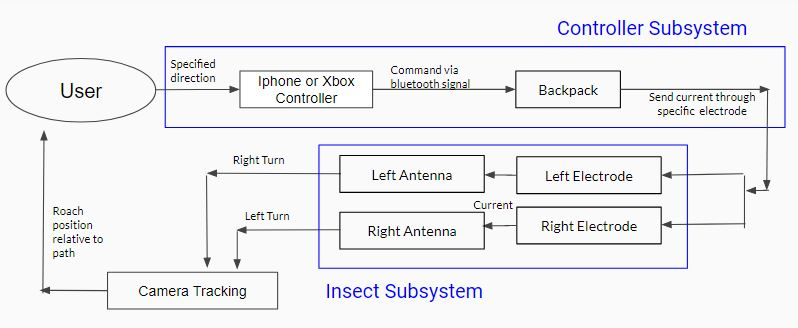
\includegraphics[scale=0.45]{fbd3.JPG}
\caption{Make Your Own RoboRoach FBD}
\label{fig:FBD3}
\end{figure}

\subsection{Decision Matrix}

\begin{figure}[ht!]
\centering
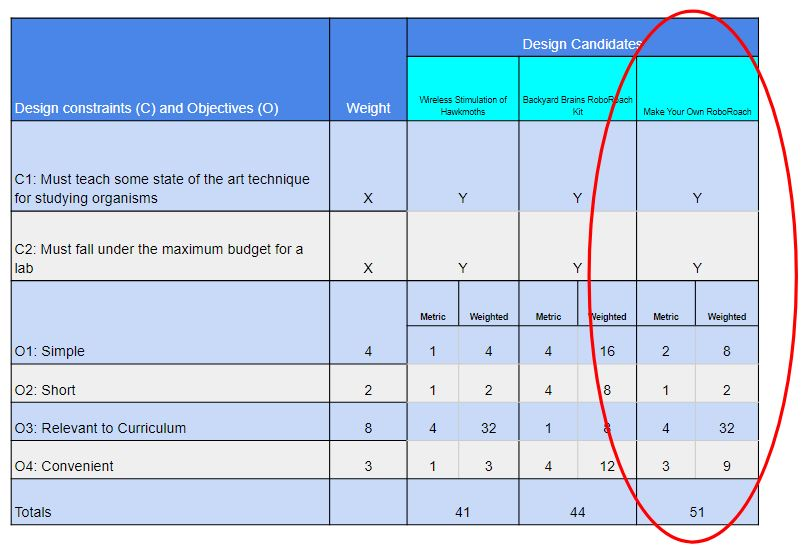
\includegraphics[scale=0.5]{decisionmatrix.JPG}
\caption{Decision Matrix}
\label{fig:DecisionMatrix}
\end{figure}

\par The decision matrix demonstrates that, with the weights designated by our customer, the Make Your Own (MYO) RoboRoach scored 51 total points whereas the moth scored 41 and the Backyard Brains kit scored 44. Although all the scores were fairly close to one another, the MYO RoboRoach ultimately won because we care most about the relevant metric, which the Backyard Brains kit fell short on. MYO RoboRoach outscored the hawkmoth because, although both offered excellent experience in scientific inquiry, the hawkmoth lab is significantly more complicated due to the additional flight aspect.

\bigskip

\par In our initial decision matrix presented in our CDR brief, our customer indicated a calculation error and reluctance to accept our "statistical significance" metric. Moving forward, we fixed the calculation error and changed "statistical significance" to "convenient" to better accommodate our vision for the learning objectives of the lab and the feasibility for the professors and students alike. After we presented our new decision matrix at our PDR brief, our customer happily approved of our winning design.

\section{Ethical Considerations}
\par Through the Backyard Brains site, we have done plenty of research on the ethical considerations for this project. Prior to performing any surgical tasks on the cockroaches, we will ensure that they are properly anesthetized. This will occur by submerging the cockroach in ice water causing them to go into a state of Hypothermia. This occurs due to the fact that cockroaches are ectothermic animals, meaning they do not produce their own heat. In this case, Hypothermia brings along a slow,light anesthesia, that causes reduced motion in the cockroach along with a diminished sensitivity of the nerves. Besides snipping the antennae in order to put the electrodes in ,little to no more invasive procedures will need to be performed on the cockroaches. We may possibly have to sand down the Pronotum of the cockroach to place the electrode connectors on it. Overall we guarantee that our cockroaches will be treated humanely during our experimentation.

\bigskip

\par This experiment also has the ability to greatly benefit future  Biomechanics studies . If we are able to fine tune the movements of the cockroach, and implement computer vision, the results of this experiment could be applied for things like reconnaissance missions in the U.S. Military. The learning outcomes could also be used in many different concentrations, including practicing controlling robots and having them execute certain tasks. 

\section{Engineering Standards and Specifications}
\par One engineering specification of our design is the connection to our PCB. Because we plan on using the TinyPico as our microcontroller, we will achieve remote control using either bluetooth or WiFi. Customer reviews indicate that the TinyPico has a tendency to overheat when using WiFi too long, so we will most likely use bluetooth for our design.

\begin{figure}[ht!]
\centering
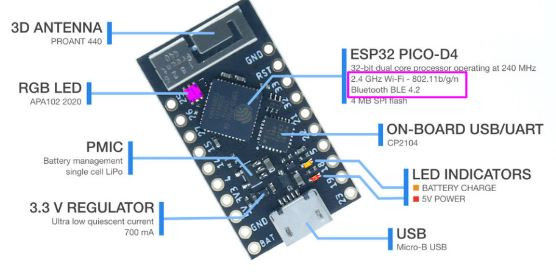
\includegraphics[scale=0.5]{ss.JPG}
\caption{TinyPico: Bluetooth and Wifi}
\label{fig:ss}
\end{figure}

\section{Preliminary Detailed Design}

\subsection{Component Selection}
\par Figure \ref{fig:morph} displays our selection of parts using a morph chart. We selected electrodes, wires, and a PCB to make the insect respond to electrical stimulus because the Backyard Brains company experience consistent success using this method. We selected a microcontroller, computer, and bluetooth as our means of creating an interface between the insect and ourselves because we knew that we'd eventually aim to achieve autonomous control over the roach, so coding on the computer would be the best way to approach that early on. Additionally, we selected bluetooth over WiFi because, as stated earlier, customer reviews of the TinyPico have noted that it overheats when WiFi is used for too long. We selected the coin cell battery over the 1S LiPo battery primarily because the coin cell was more simple but also because it is lighter than the LiPo. Although the coin cell is non-rechargeable, so we will have to buy more batteries every time the ones on hand run out of power, we felt that the coin cell was significantly less maintenance (the teachers would not have to charge the batteries before the lab) and it would be easier for us to design the PCB using the coin cell over the LiPo. Choosing the LiPo would also involve weighing different options and different corresponding headers, some of which are discontinued. The Backyard Brains RoboRoach PCB also uses a coin cell battery, so we could base our design off of theirs, the only major change being switching the main processor.

\begin{figure}[ht!]
\centering
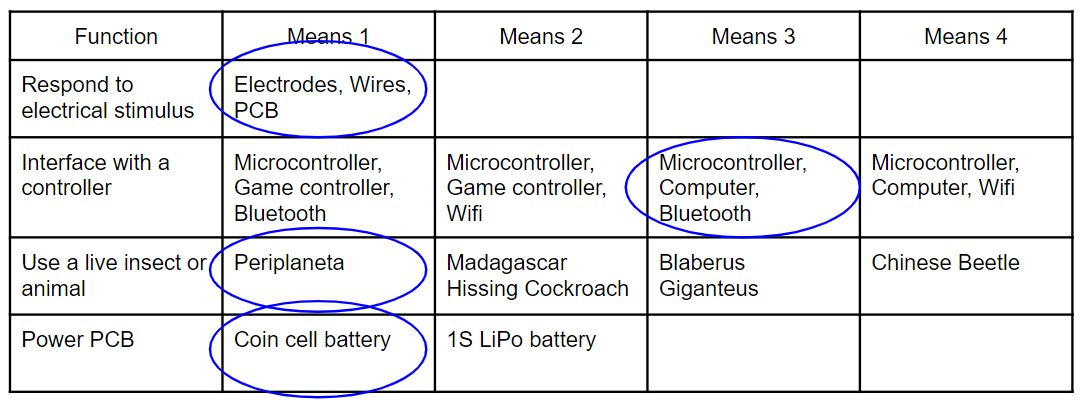
\includegraphics[scale=0.4]{morph.JPG}
\caption{Morph Chart}
\label{fig:morph}
\end{figure}

\subsection{Parts list and Budget}
As you can see from the parts list , we have a very wide array of parts needed for our project. To simplify the organization of our parts, we split them into 3 sections. The sections are Roach stuff, Make your own electrode set, and PCB backpack. The Roach stuff portion contains any parts that relate to the cockroaches specifically. This section ranges from the actual cockroaches themselves all the way to the mist bottle needed to keep the humidity in the terrarium at the proper level for the cockroaches to survive.

\bigskip

\par The next section is filled with everything needed to make the electrode sets that we will attach to the backpack and insert into the antennae of the cockroaches to create a neural interface. The last section includes everything needed for our printed circuit board backpack. The main component of this backpack will be the TinyPico, the microcontroller we will be using for this project. Other components of this section include coin cell batteries, potentiometers, double sided tape and more. The total for the parts needed for our project is \$ 642.42. We also are aware that the  cost of materials for our project may increase by up to 25\% as we change the design of our project through trial and error.

\bigskip

\par The other components that we need to take into account for our budget of our project are the Labor Cost Estimate and the Overhead Cost Estimate.  Taking into account the hours put in and the hourly pay rate for the Midshipmen, Faculty, and Staff, our subtotal for the Labor Cost of our project is \$ 14,040. For the Overhead Cost Estimate, we took 3 things into account. We looked at the Fringe Benefits, Facilities, and General Services needed to successfully execute our experimentation. The subtotal for this section also came to \$ 14,040.

\begin{figure}
\centering
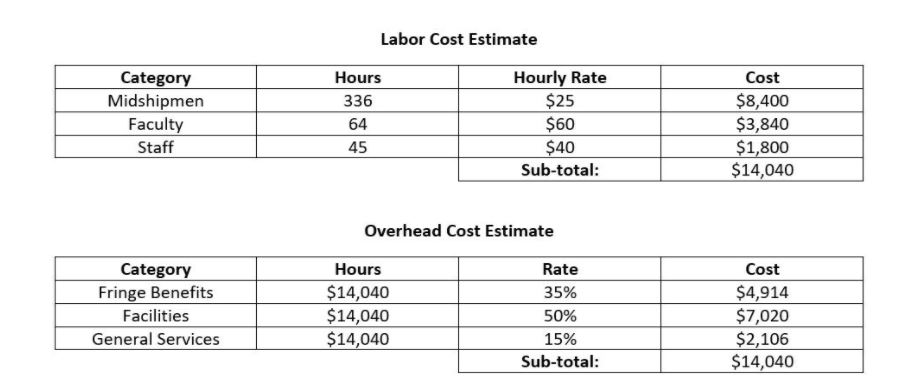
\includegraphics[scale=0.65]{budget.JPG}
\caption{Summary of Parts list}
\label{fig:budget}
\end{figure}

\begin{figure}
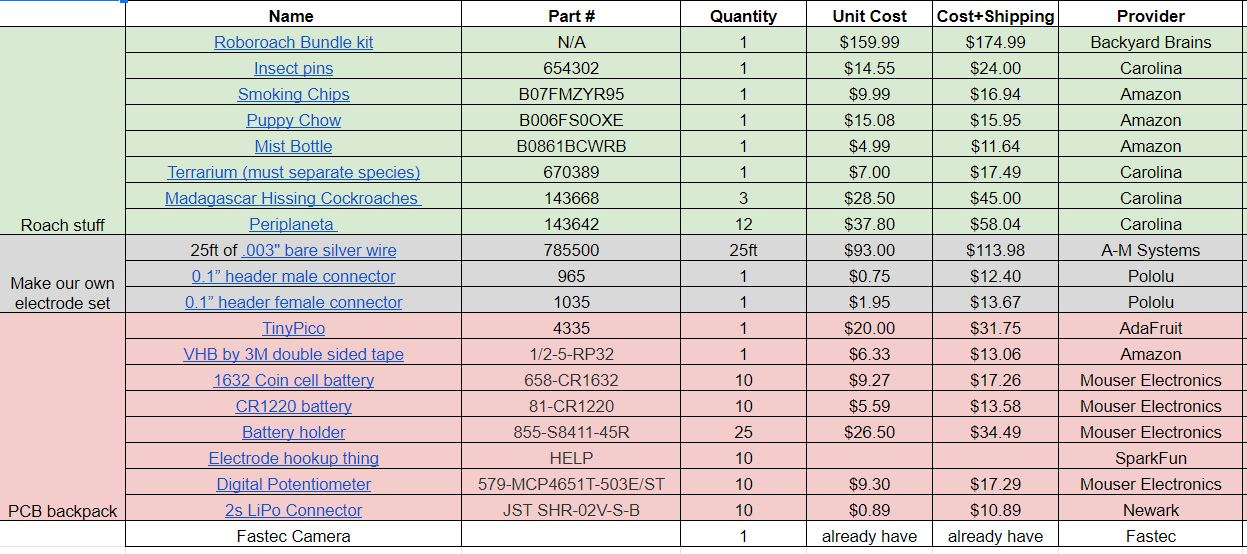
\includegraphics[scale=0.50]{partlist.JPG}
\caption{Summary of Parts list}
\label{fig:partlist}
\end{figure}

\subsection{Mechanical Drawings}
\begin{figure}[ht!]
\centering
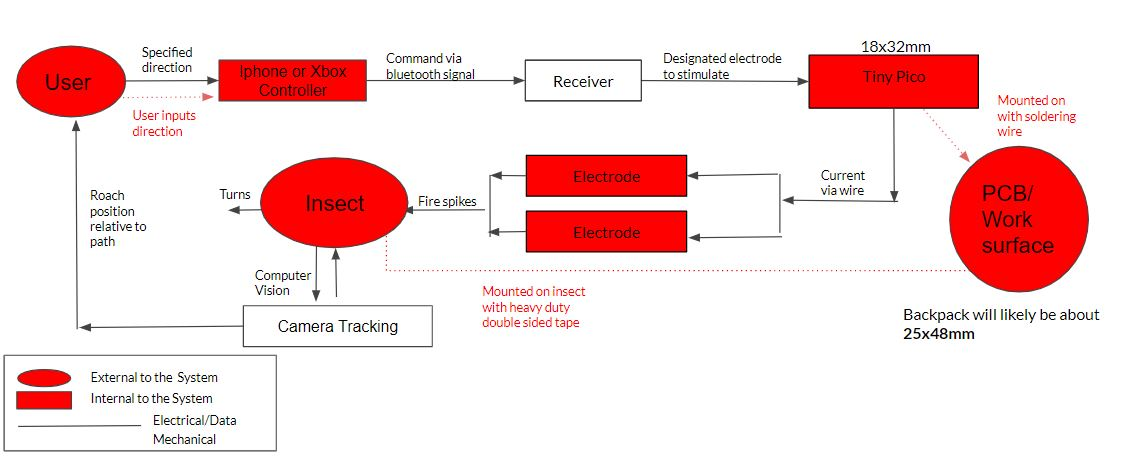
\includegraphics[scale=0.60]{mech.JPG}
\caption{Mechanical drawing of system}
\label{fig:mech}
\end{figure}

\bigskip

\par In the figure below you can see the mechanical drawing for our system. The mechanical components of our system are highlighted in red. There are also red dotted arrows that shows the relation between each of the mechanical components. The user will input which direction it wants the cockroach to turn via an Iphone or Xbox controller. The next mechanical component of the system is the Tiny Pico itself. The Tiny Pico is roughly 18x32 millimeters and will most likely be soldered to the printed circuit board by the company we choose to manufacture the board. The PCB backpack will roughly be 25x48mm and will be mounted on the insect using heavy duty double sided tape. The use of the double sided tape is for ease of removal whenever we decide to remove the backpack from a cockroach's back. Next you have the electrodes which are stuck directly into each antennae of the cockroach. The last mechanical component of our system is the cockroach itself, which will be wearing the PCB on it's back and will be responding to the electrical stimulation given to it via the electrodes that are stuck in it's antennae. 

\subsection{Circuit Diagrams}
\par Figure \ref{fig:bbs} displays the schematic for the Backyard Brains PCB, which our design is based off of. Figure \ref{fig:tps} shows the schematic for our TinyPico-based PCB design. It can be observed from the schematics that the TinyPico contains most of the necessary parts from the Backyard Brains PCB, including a processor, PIC, and LED. With the TinyPico, we only need to add a digital potentiometer, a small coin cell battery, and a connection to the electrodes that will be implanted in the antennae. The only difference in the battery circuit between the TinyPico and our design is that our design will be using a coin cell battery rather than a LiPo for power, as demonstrated in Figure \ref{fig:newbatt}.

\begin{figure}[ht!]
\centering
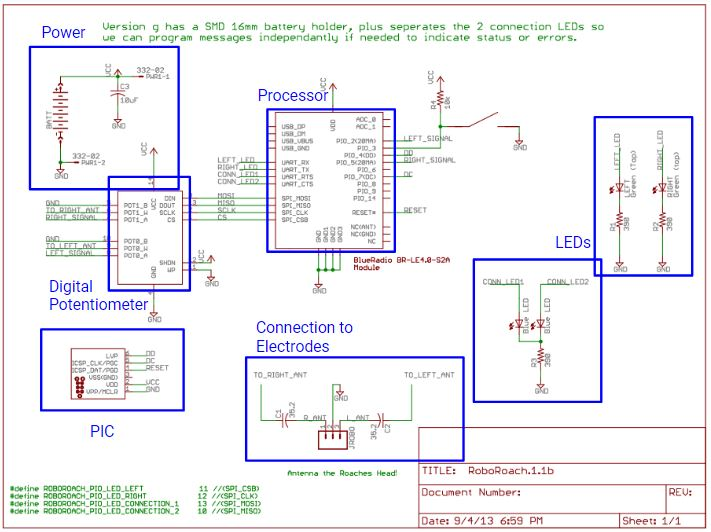
\includegraphics[scale=0.60]{BBschematic.JPG}
\caption{Backyard Brains PCB Schematic}
\label{fig:bbs}
\end{figure}

\begin{figure}[ht!]
\centering
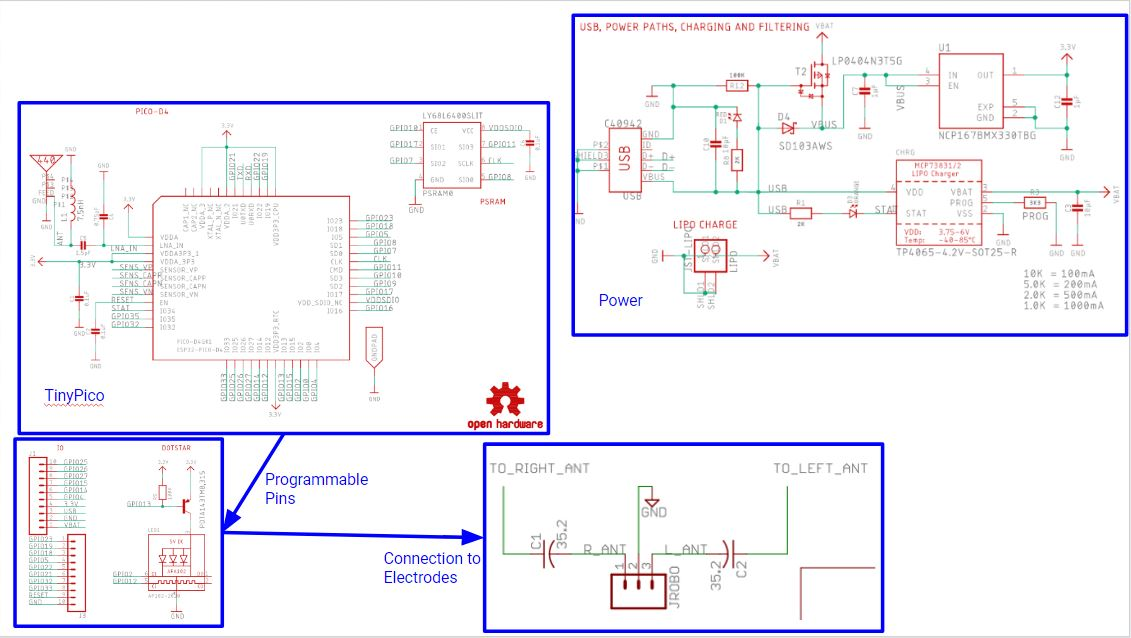
\includegraphics[scale=0.4]{TPschematic.JPG}
\caption{TinyPico-based PCB Schematic}
\label{fig:tps}
\end{figure}

\begin{figure}[ht!]
\centering
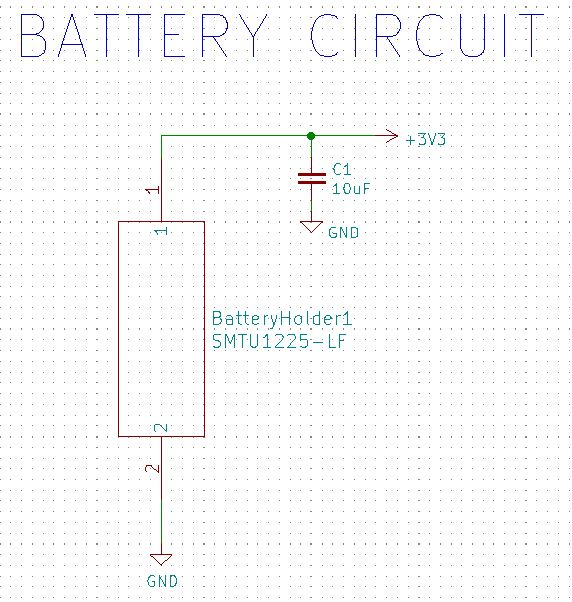
\includegraphics[scale=0.4]{Newbattery.JPG}
\caption{Our Design for a Battery Circuit}
\label{fig:newbatt}
\end{figure}

\subsection{Prototypes}
\par Figures \ref{fig:schematic}, \ref{fig:board}, and \ref{fig:3d} show demonstrate our prototype PCB concept. The backpack itself will be roughly 41x32mm in size. It will be mounted onto the cockroaches back with double sided tape. From the schematic, one can see that the components of the circuit board will mainly be the electrode base that will be connected to the electrodes implanted in the cockroaches antennae, the digital potentiometer that will regulate the curent being sent to the antennae, the battery circuit, and the TinyPico that will allow us to interface with the cockroach. We opted to keep the design fairly simple to give the students more time to focus on making a more accurate control system for their own RoboRoach. Although the 3D model looks plain right now, it will be silk screened with an aesthetically pleasing design once we have confirmed its functionality.

\begin{figure}[ht!]
\centering
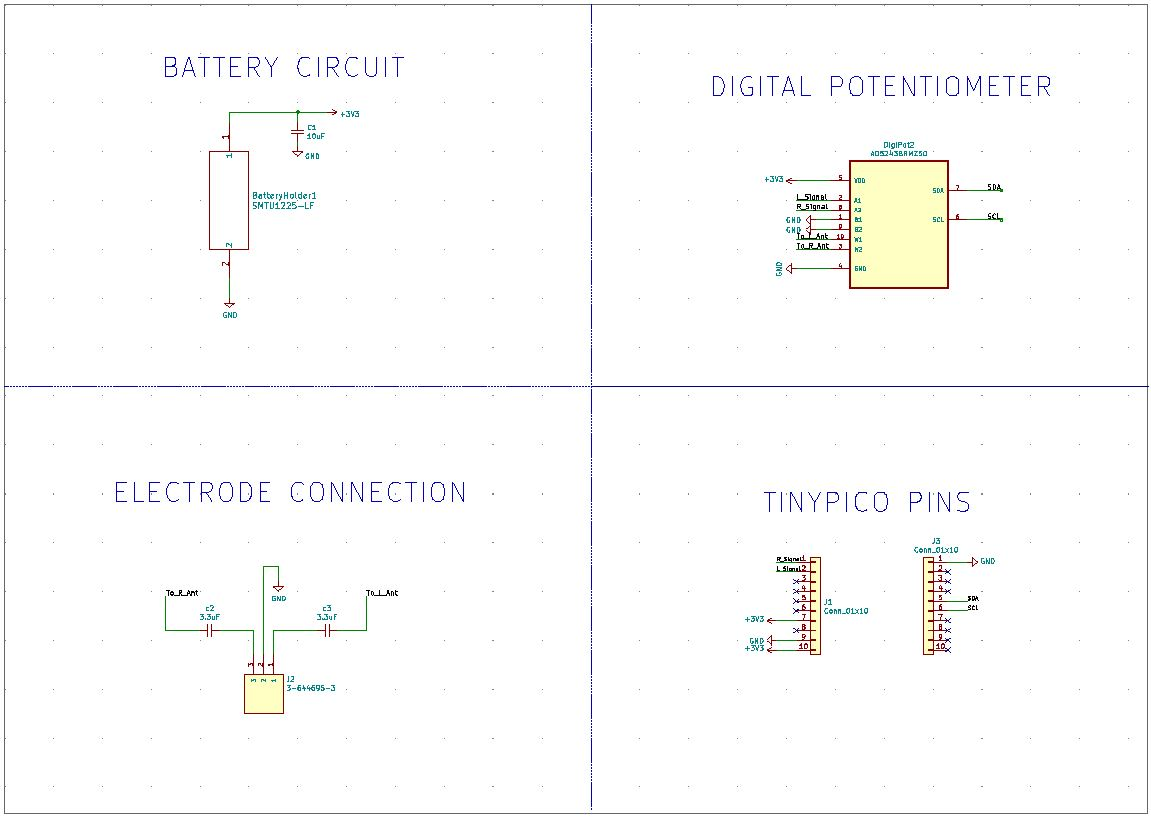
\includegraphics[scale=0.35]{EESCHEMA.JPG}
\caption{Prototype of PCB- Schematic View}
\label{fig:schematic}
\end{figure}

\begin{figure}[ht!]
\centering
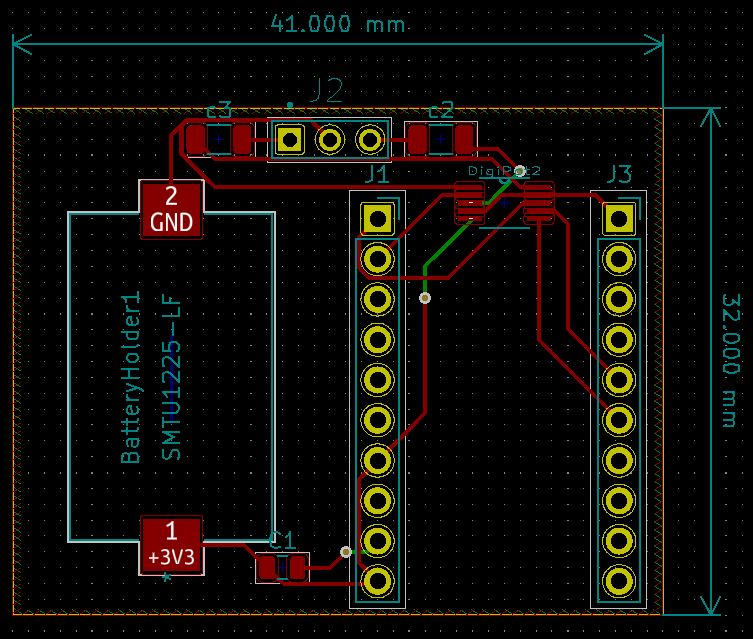
\includegraphics[scale=0.5]{myboard.JPG}
\caption{Prototype of PCB- Board View}
\label{fig:board}
\end{figure}

\begin{figure}[ht!]
\centering
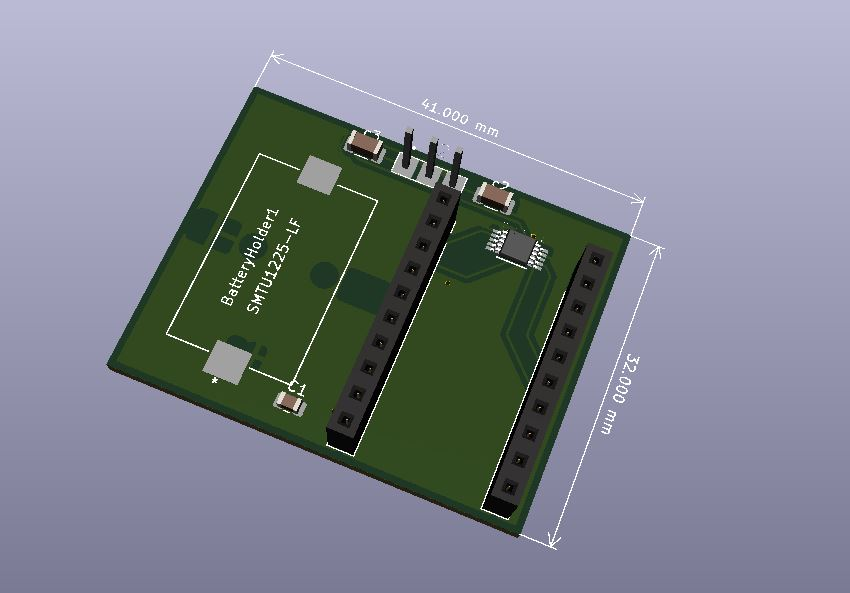
\includegraphics[scale=0.5]{my3dmodel.JPG}
\caption{Prototype of PCB- 3D Model View}
\label{fig:3d}
\end{figure}


\subsection{Software Structure}
\par Figure \ref{fig:pseudocode} displays the open loop pseudocode for our project. We plan for the user to stimulate the left antenna if he/she desires a right turn, and to stimulate the right antenna if he/she desires a left turn. If we achieve open loop control quickly, we will attempt to achieve closed loop control using computer vision, track the location of the cockroach, and compensate according to how much it is straying from the target location and in which direction.

\begin{figure}[ht!]
\centering
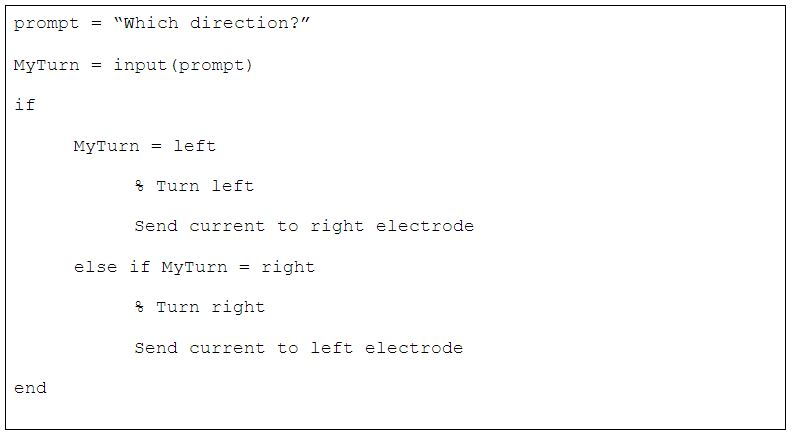
\includegraphics[scale=0.4]{pseudocode.JPG}
\caption{Open Loop Pseudocode}
\label{fig:pseudocode}
\end{figure}

\subsection{Simulations}
 ***Will discuss what simulation or other computer-aided design tools we used here- This section could include the development of a mathematical model and/or the use of a model to predict behavior and system performance.***

\section{Proposed Work}

\subsection{Work Breakdown Structure}
Looking at the functional block diagram for our system, the workload can be divided into three categories. The first of which is any work regarded the Programming for the TinyPico micro controller. The second will be anything relating to the PCB. Lastly, anything related to the cockroaches will need to be taken care of as well. Each of these will be broken down further to ensure that we have reachable goals and timelines for our project. In terms of the cockroaches, we need to construct, test, and debug the electrodes. This is an integral part of the project so it should be done early on to ensure execution of the rest of the project. Brooklyn will be charge of working with the construction and testing of the Electrodes.after construction is complete, Brooklyn will test the electrodes with an O-scope. Alexis will be in charge of the computer vision portion of the project, hoping to use camera tracking technology on the cockroaches. In terms of the TinyPico, we will write a program that will send a current to the electrodes based off of the users input. The Backyard Brains code will be available as a guide for us while we construct our code, but we are hoping to fine tune their project and will do this partially by being open to construct the code differently than theirs. This will take a large amount of testing, debugging, and documenting as we may run into differences with reactions between different cockroaches. The PCB will be a principal portion of our project. Due to the fact that we are making our own "backpack" as opposed to using the one given in the Backyard Brains RoboRoach kit, this portion of the project will be lengthy. Alexis will begin the PCB portion of our project by making a prototype on the program Eagle. This prototype will be reviewed by TSD and our capstone advisor prior to any ordering. Simultaneously, Brooklyn will be researching companies that print custom circuit boards. The decision for the PCB to be made out of house is due to the desire to have a multi-layered circuit board which cannot be easily made by TSD. Once the PCB has arrived, it will be tested to ensure it is fully working and ready to be fully implemented into the project. The care taking of the cockroaches will be split equally between Alexis and Brooklyn, as will any small tasks that come up and the final report writing.  

\subsection{Timeline}
\par Figure \ref{fig:timeline} displays the breakdown of the tasks our team needs to accomplish leading up to our final benchtop demonstration based on our WBS and general time estimates. Assuming we receive all of our ordered parts this semester and our design process goes smoothly, we should be finished creating our PCB before February and we would just have to wait for a company to send it to us.

\begin{figure}[ht!]
\centering
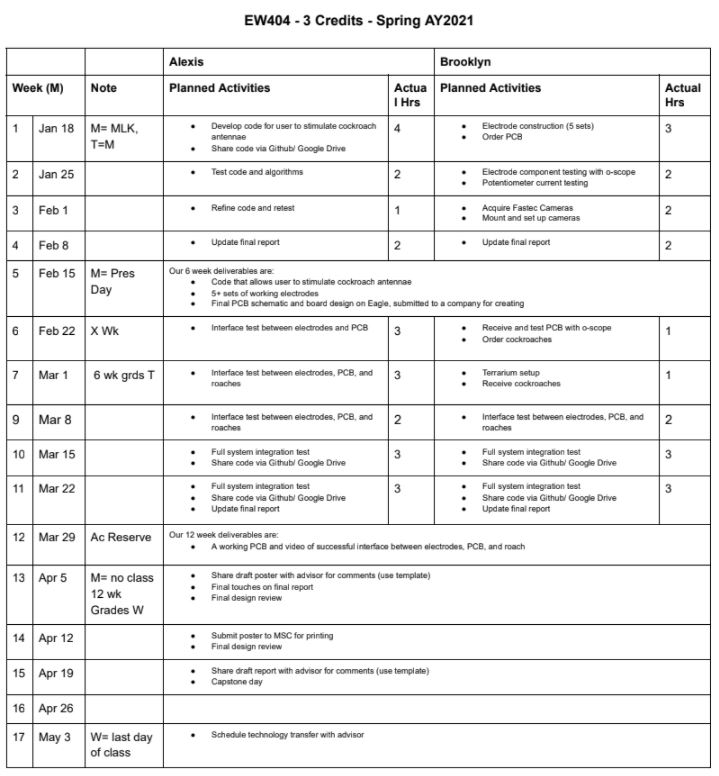
\includegraphics[scale=0.6]{TIMELINE.JPG}
\caption{Timeline and Tasks}
\label{fig:timeline}
\end{figure}

\subsection{Risk Management}
Our risks are separated into 3 categories: Technical, Business, and Programmatic. These 3 categories are designed to separate our risks by their nature.The technical category relates to things regarding technology, engineering, integration, and manufacturing.Programmatic risks relate to things regarding scheduling, staffing, communication, and estimates. Programmatic risks are all things that we can control and mitigate as a team. Lastly, Business risks are things regarding laws, resources, customers, and dependencies. These things cannot be controlled by our team. Delving into the first category, we found 2 risks that we deemed to be technical risks. 

\bigskip

\par The first technical risk relates to the design of our printed circuit board. We decided to use the program called Eagle to design our PCB prototype. Though Eagle is a widely used program for designing electrical schematics, we have never used it before. To mitigate getting behind due to the lack of experience with Eagle, we will familiarize ourselves with it as soon as possible and also reach out to TSD or other students who have prior experience with this program. With this mitigation in mind, we found this risk to be somewhat likely of occurring. The next technical risk is similar, regarding the fear of getting behind in our project due to unfamiliarity with our devices. We are using the Tiny Pico microprocessor for our project and are using python of the programming language for our coding. The unfamiliarity of both the device and the programming language may inhibit our ability to stay on schedule with the programming portion of our project. Though this is somewhat likely to happen, proper mitigation steps are taking place. Brooklyn is currently taking a python coding class, Embedded Microcontrollers, that will be applicable in terms of the coding for our project. Aside from this, Alexis will familiarize herself with the Tiny Pico schematics in order to ensure that once we receive the part, we are prepared to put it to use. 

\bigskip

\par We only have one programmatic risk- the total project budget. Though this is likely to fluctuate, it should be simple to re-evaluate each time we run into an obstacle with our project that causes us to order new parts. Because our capstone is a make-your-own version of a similar project, and is very dependent on the responses of the cockroaches to the electrical stimulation, there will be a large amount of trial and error taking place. It is likely that this causes us to order new parts, but the stress of this is mitigated by continuously checking the status of our project in order to ensure our budget does not change drastically. 

\bigskip

\par The most risks we found for our project are Business related risks. Due to this, two of the risks are extremely similar- postal delays and PCB order delays. Both of these are somewhat likely to occur, especially due to the COVID-19 Pandemic. We are aware that suppliers are experiencing delays of very unknown lengths due to COVID-19. To mitigate this, we will order our PCB from the chosen company as soon as our prototype on Eagle is both finished and approved by our project advisor. In regards to all other postal delays, we will fill out all Purchase Cards as soon as possible to ensure that our parts have plenty of leeway in the time between arrival and when they are needed. Our last risk is of the greatest impact, the possibility of being in ROM or in the online classroom environment for Capstone due to COVID-19.Though this is only somewhat likely, it will be very consequential to the fashion in which or project is executed. In order to mitigate this from greatly impacting our Capstone, we will develop a plan for online completion of our project as well as plan for a 2 week quarantine upon return to the Naval Academy in January. We will also work to complete our homework tasks early in order to allow us to get as far ahead as possible on our project. Overall, all of these risks can be mitigated with proper planning, preperation, and hard work.



\subsection{Demonstration and Testing Plan}

\par We plan to test our PCB's performance using its LED and the electrodes. Within the controller subsystem, we will evaluate its performance using the PCB's LED. If the user prompts the cockroach to turn left (port), the LED should turn red. If the user prompts the cockroach to turn right (starboard), the LED should turn green. We will know that the PCB is receiving information from the user correctly if it lights up with the color corresponding to the turn indicated by the user. Within the insect subsystem, we will evaluate its performance using the electrodes. If the user prompts the cockroach to turn left, the right electrode should receive current. If the user prompts the cockroach to turn right, the left electrode should receive current. We will know that the correct electrode is being stimulated if we observe current flowing through the selected using an oscilloscope.

\bigskip

\par The simple metric will be evaluated by the ease at which we create code to achieve open loop control. If the code is easy enough to replicate from scratch with less than a 200 course level of knowledge, this lab would earn a 4. If the code is complicated and convoluted to the point where we cannot write it without our advisor's help, this lab would earn a 0. The short metric will be evaluated by how quickly we estimate the students will be able to code and achieve open loop directional control. If the code can be completed within a lab period, we estimate that the entire lab, including surgery, programming, observation, and testing, would take 4 lab periods or fewer. However, if the code is difficult to write and requires a deeper conceptual understanding than most 200 or 300 level courses, it will likely take 5 or 6 lab periods which would earn it anywhere between a 0 and 2. The relevant metric will be evaluated by the nature of the PCB and the code we write. If, when we have successfully created a working PCB, we believe that there is a solid balance between simplicity of preparation and sufficient unknowns, the lab would earn a 4. However, if we believe that there are either too few unknowns because of how much instruction is required to execute the lab, the lab would earn a 0 or 1. The convenient metric will be evaluated by how long it takes us to build an electrode set because the professor will need to build multiple. The PCBs can be ordered in bulk well before the execution of the lab, so the only preparation the professor should need to do is build the electrode sets, order the PCBs and cockroaches, and bring all the materials to the classroom. If it takes us less than 10 minutes to build one electrode set, it would earn a 4. If it takes us more than an hour to build one, it would likely earn a 0.

\section{Benchtop Demonstration}

\subsection{Activities}
\par Through the final weeks of the semester, we used KiCAD to design our PCB, as shown in our prototype design. We studied the schematics and boards of the TinyPico and the RoboRoach PCB to investigate which pins and devices we would need. We were able to craft a schematic, board, and 3D model that can be submitted to a vendor for actual printing. We submitted our design to TSD for feedback before we order and test. We also began to interface with the TinyPico to ensure that we would not have trouble coding it.

\subsection{Results}
\par Although we were unable to produce a physical board for our audience to hold and observe, we were able to produce a design and 3D model. Once we have confirmed that the design is sound, we will order the board. We realized that the TinyPico is difficult to work with, so we have begun searching for alternative microcontrollers that are I2C compatible just in case the TinyPico ends up being too difficult to work with.

\bibliographystyle{IEEEtran}
\bibliography{roboroach.bib}
\end{document}
